\section{Przypadki uzycia}\label{sec:usecase}

\paragraph{}

Poniższy diagram przedstawia przypadki użycia aplikacji przez użytkownika. Ponieważ najważniejszym elementem aplikacji są obliczenia na karcie graficznej, oraz wyświetlanie ich wyników w przyjaznej dla oka formie, główną aktywnością użytkownika jest oglądanie efektów obliczeń i cieszenie oka efektami specjalnymi. Jednak aby aplikacja była choć trochę funkcjonalna, użytkownikowi umożliwione będzie podstawowa kontrola symulacji.

\begin{figure}[h]
	\centering
	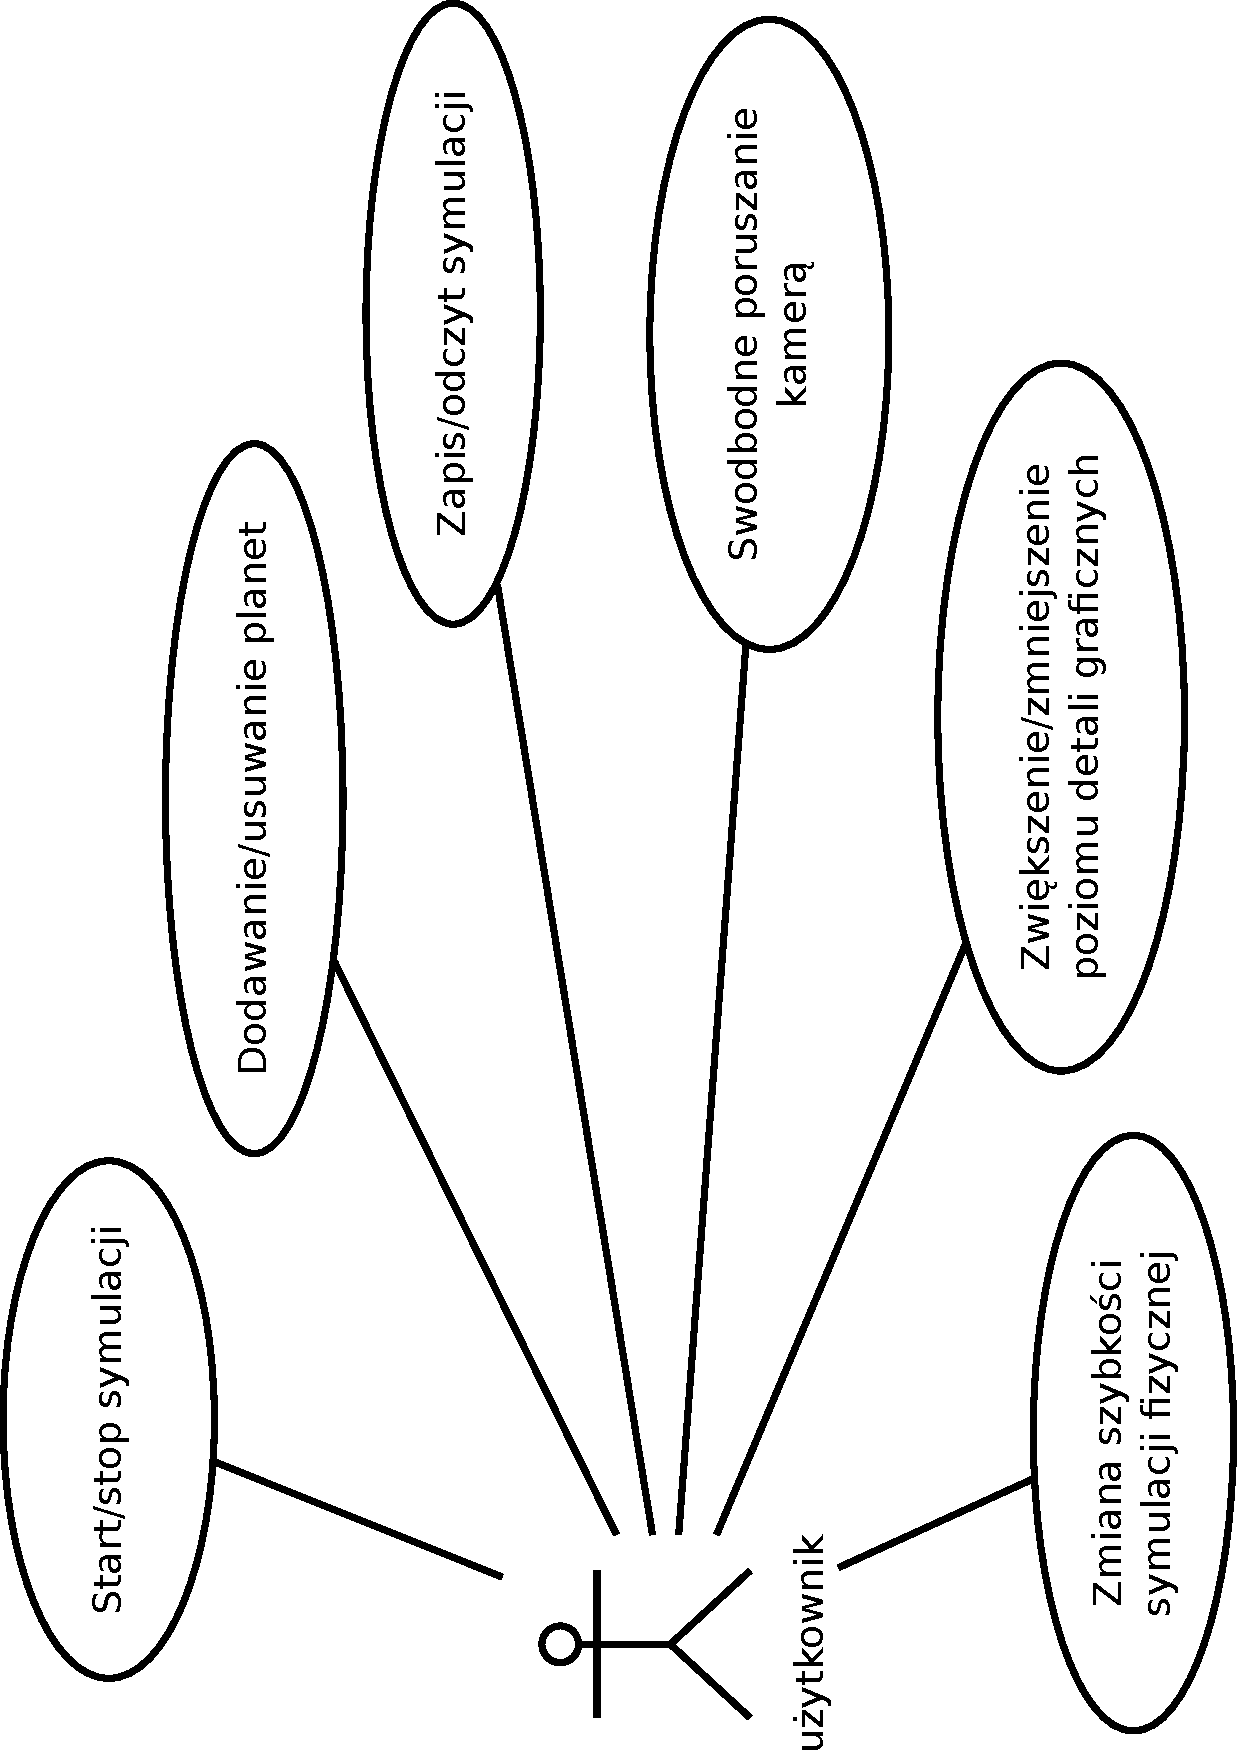
\includegraphics[width=0.5\textwidth,angle=-90]{use-case.pdf}
	\caption{Diagram przypadków użycia}
	\label{fig:use-case}
\end{figure}

\paragraph{}

Znaczenie poszczególnych przypadków użycia dla aplikacji jest następujące:

\begin{description}
	\item[Start/stop symulacji] - aplikacja powinna przewidywać możliwość zatrzymania i wznowienia symulacji fizycznej, nie blokując przy tym możliwości poruszania kamera. W trybie pauzy powinna być również możliwość dodawania/usuwania planet.
	\item[Dodawanie/usuwanie planet] - aby dać użytkownikowi możliwość budowania własnych układów, aplikacja powinna pozwalać na usuwanie planet uczestniczących w aktualnej symulacji, oraz na dodawanie nowych planet, nadając im masę, pozycje, oraz prędkość początkowa. Wygodnym sposobem ustawiania nowej planety jest używanie myszki, dla ustalenia pozycji, oraz prędkości początkowej.
	\item[Zapis/odczyt symulacji] - aplikacja powinna pozwalać na wczytywanie wcześniej zdefiniowanych układów, ponieważ uzyskanie stabilnego układu planetarnego nie jest rzeczą prostą. Jeśli jednak sie to uda, powinna być również możliwość zapisania aktualnego stanu symulacji.
	\item[Swobodne poruszanie kamera] - swobodna kamera oznacza, ze można przesuwać ja w dowolnym kierunku, tak aby była możliwość ustawienia jej w dowolnej pozycji, oraz można ja obracać w dowolna stronę. Na przesuwnie kamery najwygodniej pozwolić za pomocą klawiszy klawiatury, natomiast obroty najwygodniej realizuje sie poprzez ruch myszki.
	\item[Zmiana poziomu detali graficznych] - w zależności od mocy karty graficznej na maszynie wywołującej program, powinna być możliwość ustawienia szczegółowości prezentowanej symulacji. Miedzy innymi można sterować ilością wierzchołków składających sie na obiekt (teselacja), rozdzielczością oraz sposobem mapowania tekstur, ilością prezentowanych efektów specjalnych, ilością gwiazd (źródeł światła).
	\item[Zmiana szybkości symulacji fizycznej] - w zależności od możliwości jednostki graficznej na której dokonywane są obliczenia fizyczne, można ustawić więcej, bądź mniej klatek fizycznych na jedna klatkę graficzna, tak aby uzyskać tak samo dokładną symulacje w krótszym czasie.
\end{description}

